\documentclass[border=2pt]{standalone}

% Drawing
\usepackage{tikz}

% Define Color
\definecolor{g1}{rgb}{0.0, 1.0, 0.0}

% Tikz Library
\usetikzlibrary{angles, patterns, quotes, calc, decorations.markings, decorations.pathmorphing}

% Tikz Style
\tikzset{every node/.style={align=center}}
\tikzset{arrow inside/.style = {postaction=decorate,decoration={markings,mark=at position .52 with \arrow{stealth}}}}
\tikzset{ray/.style={very thick, red, arrow inside}}
\tikzset{line/.style={thick, black}}
\tikzset{lined/.style={thick, black, dashed}}

% New Command
%% To Draw the Reflector and the Perpendicular Line to It
\newcommand{\cdraw}[3]{\draw[#3] (-{#1*cos(#2)}+4, -{#1*sin(#2)+4}) -- ({#1*cos(#2)+4}, {#1*sin(#2)+4})}
%% To Draw the Viewing Screen
\newcommand{\cdraww}[3]{\draw[#3] (-{#1*cos(#2)}+7.5, -{#1*sin(#2)+1}) -- ({#1*cos(#2)+7.5}, {#1*sin(#2)+1})}
%% To Fill with North West Lines in Polar Coordinates
\newcommand{\cfill}[2]{\fill[pattern = north west lines]
 (-{#1*cos(#2)}+4, -{#1*sin(#2)+4}) -- 
 ({#1*cos(#2)+4}, {#1*sin(#2)+4}) -- 
 ({#1*cos(#2)+3.8}, {#1*sin(#2)+3.8}) --
 (-{#1*cos(#2)+3.8}, -{#1*sin(#2)+3.8}) -- 
 (-{#1*cos(#2)+4}, -{#1*sin(#2)+4}) -- cycle}

\begin{document}
	
	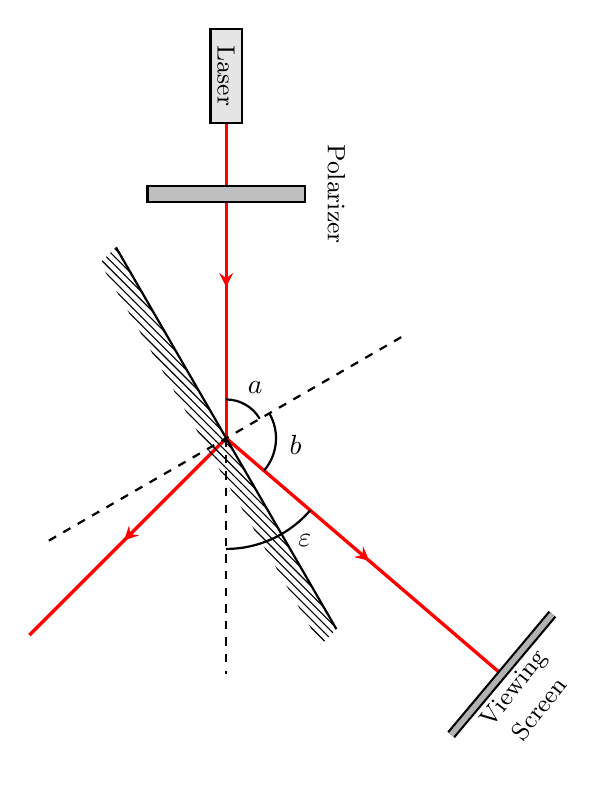
\begin{tikzpicture}	
%		% Grid
%		\draw[dotted, black!30] (0,0) grid (10,10);
%		\foreach \i in {0,...,10}
%		{
%			\node at (-2ex,\i) {\i};
%			\node at (\i,-2ex) {\i};
%		}
		
		% Coordinates
		\coordinate (O) at (4,4);
		\coordinate (P) at (4,8);
		\coordinate (P') at (4,1);
		\coordinate (A) at (7.5,1);
		\coordinate (D) at (1.5,1.5);
		\coordinate (G) at ({4+3*cos(120)},{4+3*sin(120)});
		\coordinate (G') at ({4-3*cos(120)},{4-3*sin(120)});
		\coordinate (K) at ({4+3*cos(30)},{4+3*sin(30)});
		\coordinate (K') at ({4-3*cos(30)},{4-3*sin(30)});
		%% Coordinate Visulization
%		\point{A}{$A$}{right}
%		\point{O}{$O$}{left}
%		\point{P}{$P$}{right}
%		\point{P'}{$P'$}{right}
%		\point{D}{$D$}{right}
%		\point{G}{$G$}{right}
%		\point{G'}{$G'$}{right}
%		\point{K}{$K$}{right}
%		\point{K'}{$K'$}{right}

		
		% Rays
		\draw[ray] (P) -- (O);
		\draw[ray] (O) -- (A);
		\draw[ray] (O) -- (D);
		%% Dashed
		\draw[lined] (O) -- (P');
		
		% Reflector
		\cdraw{2.8}{120}{line};
		\cfill{2.8}{120};
		%% Dashed
		\cdraw{2.6}{30}{lined};
		
		% Angles
		\pic[draw, thick, angle radius=14pt, angle eccentricity=1.5pt, "$a$"] {angle=K--O--P};
				\pic[draw, thick, angle radius=18pt, angle eccentricity=1.4pt, "$b$"] {angle=A--O--K};
		\pic[draw, thick, angle radius=40pt, angle eccentricity=1.5pt] {angle=P'--O--A};
		\node at (5,2.7) {$\varepsilon$};
		
		% Polarizer
		\draw[thick, fill=black!25] (3,7.2) rectangle (5,7);
		%% Node
		\node[rotate=270] at (5.4, 7.1) {\small Polarizer};
		
		% Viewing Screen
		\cdraww{1}{50}{line, black, double distance = 2pt, double = black!30};
		%% Node
		\node[rotate=52] at (7.8,0.7) {\small Viewing\\\small Screen};
		
		% Layser
		\draw[thick, fill=black!10] (3.8,9.2) rectangle (4.2,8);
		%% Node
		\node[rotate=270] at (4,8.6) {\small Laser};
	\end{tikzpicture}
	
\end{document}